\section{The model}\label{sec:model}

\subsection{Material, placement, and regularity}

Paper is modelled as an inextensible surface of zero thickness. For $0<w<L$ the \emph{strip} is the rectangle $R_{L,w}=[0,L]\times[-\tfrac w2,\tfrac w2]$ carrying the Euclidean metric; all the information the material holds at this stage is intrinsic, namely lengths and angles measured along the sheet. The sheet has zero material thickness throughout. Non-penetration means injectivity of the realized surface, and $\varepsilon$ bounds the height of its containing slab; it is neither material thickness nor a minimum separation between sheets. A positive-thickness material model would require additional assumptions.

\begin{definition}[Admissible configuration]\label{def:admissible}
A map $F\colon R_{L,w}\to\R^3$ is \emph{inextensible} where it is differentiable if $(DF)^{T}DF=I_2$, equivalently if it preserves the length of every material curve. It is an \emph{admissible configuration} if there is a finite graph $\Gamma\subset R_{L,w}$, the \emph{crease pattern}, such that $F$ is a $C^2$ inextensible immersion on every connected component of $R_{L,w}\setminus\Gamma$, called a \emph{panel}, and $F$ is continuous on all of $R_{L,w}$.
\end{definition}

\begin{remark}[The regularity class is a modelling decision]\label{rem:regularity}
Inextensibility alone forces nothing. By the Nash--Kuiper theorem \cite{nash1954,kuiper1955} a $C^1$ isometric embedding of a strip exists inside a ball of arbitrarily small radius, so paper-likeness is not a consequence of not stretching. It is the class of Definition~\ref{def:admissible}, piecewise $C^2$ with finitely many creases, that makes the Gauss curvature argument available on panels, so that a panel is developable, hence ruled \cite{docarmo1976}, and flat states are rigid. Every theorem below is a theorem about this class.
\end{remark}

On a \emph{flat} configuration the class collapses to something completely rigid: each panel is a rigid piece of the plane, each crease is a straight line, and adjacent panels are related by reflection in that line. This is a structure theorem, not a definition, and it has one consequence that organizes the whole paper: the continuous information carried by a flat folded state is exactly the positions of the creases, and everything else is combinatorial. That is why a finite-dimensional coordinate chart exists at all (Proposition~\ref{prop:dim}).

\subsection{Long strips, flat folded states, and diagrams}

To speak of knotting we replace the finite strip by the long strip $R_w=\R\times[-\tfrac w2,\tfrac w2]$. A \emph{long-strip placement} is an admissible configuration $F\colon R_w\to\R^3$ with finite bounded crease pattern whose image agrees, outside some ball, with two straight half-infinite flat ribbons. Admissibility asks immersion, not injectivity, so a placement's centreline may self-intersect; a placement whose centreline is injective---then automatically a proper embedding, being straight outside a ball---is a \emph{spatial long-strip knot configuration}, a \emph{long-strip configuration} for short. The \emph{knot type} of a spatial long-strip knot configuration is the ambient-isotopy class of its centreline, a classical long knot; planar folded states, whose centrelines self-intersect by design, are assigned no spatial knot type directly, their tiedness being the diagrammatic one used throughout; the ribbon carries strictly more data---framing, annulus versus M\"obius after closure---which Remark~\ref{rem:framing} records and which this paper does not use. The two straight ends are the topological substitute for holding the strip in one's hands: a knot cannot escape off the end. The price is that the existence threshold, that is how long a strip must be before a given knot can be tied in it, is excluded from the model; that question belongs to ribbonlength theory \cite{kauffman2004,denne2020,chen2025} and is not treated here.

\begin{proposition}[Long knots and their closures]\label{prop:closure}
The centreline of a spatial long-strip knot configuration is, by definition, a proper embedding $\gamma\colon\R\hookrightarrow\R^3$ that is straight outside a ball; adding the point at infinity extends it canonically to an embedding $\bar\gamma\colon S^1\hookrightarrow S^3=\R^3\cup\{\infty\}$, tame at $\infty$ because the two tails are straight. Centreline knot types of long-strip configurations correspond bijectively, via $\gamma\mapsto\bar\gamma$, to classical closed knot types.
\end{proposition}

\begin{proof}
Compactness at infinity makes the closure canonical: the one-point compactification requires no choice of closing arc, and an ambient isotopy of $\R^3$ through long-strip configurations, being straight outside a ball, extends to an ambient isotopy of $S^3$ fixing $\infty$. Conversely every classical knot type contains a representative straight outside a ball, which reads back as a long-strip centreline.
\end{proof}

\begin{remark}[Framing ledger]\label{rem:framing}
A ribbon carries more than its centreline: whether the closed-up ribbon is an annulus or a M\"obius band is determined by the parity of the crease number together with the writhe of the diagram. This is bookkeeping parallel to, and not part of, the knot type, and it is not used below.
\end{remark}

\begin{definition}[Flat folded state]\label{def:flatstate}
A \emph{flat folded state} is a pair $(f,\lambda)$ in which $f\colon R_w\to\R^2$ is a planar long-strip placement all of whose creases are \emph{complete}, meaning that in material coordinates each crease is a chord joining the two long edges and hence crosses the centreline, and $\lambda$ is a \emph{layer order}: a local linear order on the material points sharing a plane point, subject to the standard non-crossing axioms of flat origami \cite{justin1997,hull2002,demaine2007}. The instance of those axioms used in this paper is Definition~\ref{def:axiom}.
\end{definition}

\begin{definition}[Tying data]\label{def:tying}
Erasing the continuous information from a flat folded state leaves the combinatorial type $(n,\epsilon_1\cdots\epsilon_n,\lambda)$, where $n$ is the number of creases in material order, $\epsilon_i\in\{+,-\}$ is the \emph{tilt sign}, also called the crease-slope sign, of crease $i$, and $\lambda$ is the combinatorial layer order. The space of flat folded states realizing a given tying datum is its (honest) moduli space; for the overhand branch, Section~\ref{sec:moduli} names it $\Mhon$ and fixes the working subspaces $\Mplus\subseteq\Mhat$ used throughout.
\end{definition}

The basic split of the theory is contained in that definition: the tying is a discrete datum, a shape is a point of the honest moduli $\Mhon$, and tightening is a motion inside it; the optimization of this paper is carried out on the working chamber $\M=\Mhat$, with the local theorems taking place in $\Mplus$ (Section~\ref{sec:moduli}); Figure~\ref{fig:notation} displays the two sides of the split.

\begin{figure}[t]
\centering
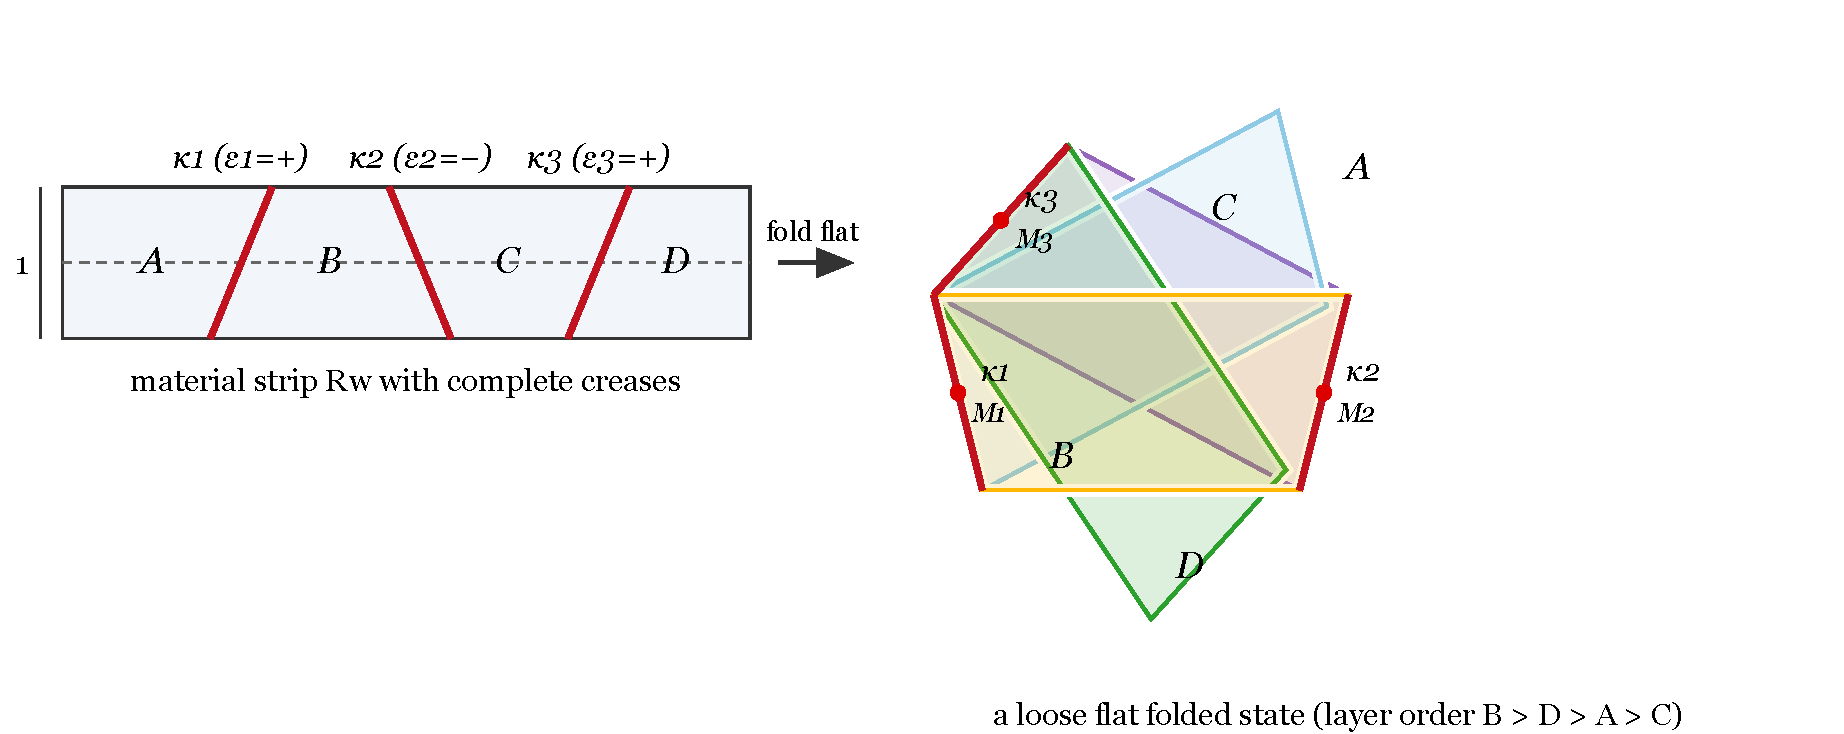
\includegraphics[width=0.98\linewidth]{figs/fig0-notation.pdf}
\caption{The split into tying and shape. Left: material coordinates---the long strip $R_w$, three complete crease chords $\kappa_1,\kappa_2,\kappa_3$ with tilt signs $\epsilon$, and the passes $A,B,C,D$ they bound. Right: a loose flat folded state of the overhand branch realizing this datum, drawn from exact slice coordinates: panels are rigid, creases (heavy) are straight chords with fold points $M_i$ on the centreline, and the layer order $B>D>A>C$ decides every crossing.}
\label{fig:notation}
\end{figure}

\begin{observation}\label{obs:diagram}
A flat folded state \emph{is} a knot diagram. The image of the centreline is a planar polyline, straight on each panel by rigidity; in general position its self-intersections are finitely many transverse double points, and at each of them the layer order $\lambda$ of the two panels involved decides which strand is over. Thus $(f,\lambda)$ determines a long-knot diagram $D(f,\lambda)$ with no auxiliary projection and no further interpretation.
\end{observation}

We call $(f,\lambda)$ \emph{tied} if $D(f,\lambda)$ represents a nontrivial knot type.

\begin{remark}[Crease mobility]\label{rem:mobility}
A tightening path varies the positions \emph{and} the angles of the creases continuously, preserving only the crease number and the combinatorial datum. The creases of this model are therefore movable fold lines, idealized lines of concentrated curvature that roll along the material, and not plastic scars pinned to material coordinates. The pinned-crease model and the refolding model, in which an existing crease is undone and a new one made, are different problems, and any comparison with a physical experiment must say which model is meant.
\end{remark}

\subsection{The fold number and the rigidity of the tying}

Throughout this subsection $(f,\lambda)$ is a flat folded state with $n$ complete creases, whose centreline pieces are $P_0,\dots,P_n$, with $P_0$ and $P_n$ rays and the rest segments.

\begin{definition}[General position]\label{def:gp}
The state is in \emph{general position} (GP) if no two pieces overlap in more than one point, and all double points of the centreline are transverse, pairwise distinct, and at positive distance from fold points and crease segments.
\end{definition}

General position is not an extra hypothesis imposed for convenience. It is precisely the condition under which the diagram of Observation~\ref{obs:diagram} is well defined, and being tied presupposes that diagram; a degenerate fold angle, for instance, produces a collinear overlap of adjacent pieces and is excluded by the first clause. In this sense a tied state means, by definition, a state in general position.

\begin{remark}[Numerical remark]\label{rem:gpaudit}
The general-position margins are comfortable at every state we have examined. At the regular pentagon the minimum crossing angle is $72.0^\circ$ and the smallest crossing-to-crease distance is $0.500$ in units of the strip width; at the tight state $\td$ the corresponding values are $69.5^\circ$ and $0.517$, and at a loose slice state $56.1^\circ$ and $0.658$. Over $2000$ random valid states the minimum crossing angle is $28.4^\circ$ and the crossing-to-crease distance never drops below $0.506$; in every state audited the crossing pairs are exactly $\{(P_0,P_2),(P_0,P_3),(P_1,P_3)\}$, with no adjacent-pair crossing and no collinear pair. These are numerical audits, recorded in the ancillary verification suite \cite{anc}.
\end{remark}

\begin{lemma}[Straightness and the crossing bound]\label{lem:crossbound}
Under GP the crossings of $D(f,\lambda)$ are exactly the transverse double points of non-adjacent pairs of pieces, and each such pair crosses at most once. Hence the number of crossings is at most $\binom{n+1}2-n=\tfrac{n(n-1)}2$.
\end{lemma}

\begin{proof}
Each panel is rigid, so $P_i\subset\Lambda_i$ for a line $\Lambda_i$ and no piece meets itself. Two distinct lines meet at most once, and GP makes the meeting transverse. For an adjacent pair, $\Lambda_{i+1}=\rho_i(\Lambda_i)$ with $\rho_i$ the reflection in the crease line $\ell_i$, and the fold point $M_i\in\Lambda_i\cap\ell_i$ is fixed by $\rho_i$, so $M_i\in\Lambda_i\cap\Lambda_{i+1}$. If $\Lambda_{i+1}\ne\Lambda_i$ this is their only intersection, and it is a fold vertex shared as an endpoint rather than a double point. The remaining case $\Lambda_{i+1}=\Lambda_i$ means $\rho_i(\Lambda_i)=\Lambda_i$, hence either $\Lambda_i=\ell_i$, which is impossible because a complete crease is a chord joining the two long edges and is therefore transverse to the centreline, or $\Lambda_i\perp\ell_i$, a perpendicular fold-back in which two adjacent pieces overlap collinearly and which GP excludes.
\end{proof}

In particular $n\le2$ permits at most one crossing, and $n=3$ at most three.

\begin{lemma}[Crossing-preserving closure]\label{lem:closureop}
Let $\Delta$ be a disc containing all creases and all crossings in its interior. Then $D\setminus\Delta$ consists of two straight tails, each meeting $\partial\Delta$ once and transversally; joining the two cut points by an arc of $\partial\Delta$ produces a closed generic curve $\widehat D$ with no new crossings, whose knot type is the closure of the long knot represented by $D$ and whose Gauss code, read cyclically, is unchanged.
\end{lemma}

\begin{proof}
Choose the radius large enough that all fold points and crossings lie in the interior. The disc is convex, so the intermediate segments, whose endpoints are interior fold points, lie wholly inside it, while each of the two rays leaves from an interior point, crosses $\partial\Delta$ exactly once transversally, and stays outside afterwards. Hence the only intersections of the tails with $\partial\Delta$ are the two cut points, and the interior of the joining arc misses $D$ entirely. Independence of the closure is Proposition~\ref{prop:closure}.
\end{proof}

\begin{lemma}[Gauss parity]\label{lem:parity}
In the Gauss code of a closed generic plane curve, the number of symbols strictly between the two occurrences of any given symbol is even.
\end{lemma}

\begin{proof}
A crossing $c$ splits the curve into two closed loops $\gamma_1,\gamma_2$. In a cyclic code it does not matter which of the two arcs is counted, since the two counts differ by an even number. The symbols between the two occurrences of $c$ are the crossing events on $\gamma_1$; a self-crossing of $\gamma_1$ contributes two such events and a crossing with $\gamma_2$ contributes one, so the parity in question equals $|\gamma_1\cap\gamma_2|\bmod2$. Rounding the corner at $c$ separates $\gamma_1$ and $\gamma_2$ near $c$ into two transverse closed curves, and two closed curves in the plane meet in an even number of points, the $\mathbb Z/2$ intersection number vanishing by the Jordan curve theorem.
\end{proof}

\begin{lemma}[At most two crossings implies unknotted]\label{lem:twocrossings}
A long or closed diagram with at most two crossings represents the trivial knot; hence a nontrivial knot satisfies $c(K)\ge3$.
\end{lemma}

\begin{proof}
Close the diagram up by Lemma~\ref{lem:closureop}. With one crossing the code is $XX$. With two crossings the cyclic code is, up to renaming, of type $XXYY$, which contains an adjacent repeat, or $XYXY$; the latter has exactly one symbol, an odd number, between the two occurrences of $X$, and is excluded by Lemma~\ref{lem:parity}. Every remaining code has an adjacent repeat, so some crossing is traversed twice consecutively and the loop between the two passages carries no crossing event. That loop is an embedded Jordan curve, and the rest of the curve is a connected set meeting it only at the vertex, so one of the two complementary discs is free of the diagram; a first Reidemeister move across that disc on $S^2$ removes one crossing. Induction terminates at zero crossings. The underlying enumeration of codes is also machine-checked in the ancillary verification suite \cite{anc}.
\end{proof}

\begin{lemma}[Passage order for three creases]\label{lem:passage}
Let $n=3$ and suppose the three non-adjacent pairs $X=(P_0,P_2)$, $Y=(P_0,P_3)$ and $Z=(P_1,P_3)$ each cross exactly once. In material coordinates the passages follow the block order $P_0<P_1<P_2<P_3$, so the only freedom is the order of the two passages inside $P_0$ and of the two inside $P_3$, giving four codes. Exactly one of them is realizable in the plane, namely $\mathtt{XYZXYZ}$.
\end{lemma}

\begin{proof}
Apply Lemma~\ref{lem:parity} to the closed code. In $\mathtt{YXZXYZ}$ there are three symbols, $X,Z,X$, between the two occurrences of $Y$; in $\mathtt{XYZXZY}$ likewise three between the two occurrences of $Y$; and $\mathtt{YXZXZY}$ has one between the two occurrences of $X$. Only $\mathtt{XYZXYZ}$ has an even count, namely two, for every symbol.
\end{proof}

\begin{lemma}[Shadow rigidity]\label{lem:shadow}
The shadow of any closed realization of $\mathtt{XYZXYZ}$, that is the four-valent plane graph obtained by forgetting over and under, is unique on $S^2$ up to homeomorphism and mirror, and equals the shadow of the closure of the two-strand braid $\sigma_1^3$.
\end{lemma}

\begin{proof}
There are three vertices of valence four and six edges, hence five faces on $S^2$. The code has no adjacent repeat, so there are no loop edges and no monogons: every face has degree at least two and the degrees sum to $12$. Absence of loops gives, at each vertex, $m_{XY}+m_{XZ}=m_{XY}+m_{YZ}=m_{YZ}+m_{XZ}=4$, whence $m_{XY}=m_{YZ}=m_{ZX}=2$, a doubled triangle. A bigon face consumes both edges of one pair, so there are at most three bigons; the degree partition $(2,2,2,2,4)$ is therefore impossible and $(2,2,2,3,3)$ holds, giving exactly three bigons and two triangles. Transversality at a four-valent vertex pairs opposite half-edges into the same strand, since two strands can cross only if the two ends of one separate the two ends of the other. Collapsing each bigon to a single fat edge yields an embedding of the triangle $XYZ$ in $S^2$, unique up to homeomorphism, and the expansion back is unique as well; the result is the shadow of the closure of $\sigma_1^3$, with its three bigons and two triangles. The complementary enumeration of rotation systems, in which transversality allows two at each vertex and hence eight in all, of which exactly two are planar with face vector $(2,2,2,3,3)$ and are vertexwise reversals of one another, is machine-checked in the ancillary verification suite \cite{anc}.
\end{proof}

\begin{theorem}[Fold number and rigidity of the tying]\label{thm:foldnumber}
Let $(f,\lambda)$ be a tied flat folded state in general position. Then it has at least three creases. If it has exactly three, then the three non-adjacent piece pairs cross exactly once each and there are no other crossings; the material passage order is forced to be $\mathtt{XYZXYZ}$; the over-under resolution must be alternating, and there are exactly two possibilities, mirror images of one another; and the knot type is the left- or right-handed trefoil. In particular the entire crossing combinatorics, that is which pairs cross, in which material order, and with which over and under, is unique up to mirror.
\end{theorem}

\begin{proof}
If $n\le2$ there is at most one crossing by Lemma~\ref{lem:crossbound}, hence the state is unknotted by Lemma~\ref{lem:twocrossings}, contradicting tiedness. Suppose $n=3$. Tiedness and Lemma~\ref{lem:twocrossings} force at least three crossings and Lemma~\ref{lem:crossbound} forces at most three, so there are exactly three, one per non-adjacent pair. Lemma~\ref{lem:passage} forces the code $\mathtt{XYZXYZ}$, and Lemma~\ref{lem:shadow} identifies the shadow with that of the closure of $\sigma_1^3$, so the diagram is the closure of $\sigma_1^{s_1}\sigma_1^{s_2}\sigma_1^{s_3}$ for signs $s_j\in\{\pm1\}$, up to homeomorphism of $S^2$ and mirror.

Mixed signs are impossible. If $(s_j)$ is not constant, the word contains an adjacent pair of opposite signs; then $\sigma_1^{+1}\sigma_1^{-1}$ cancels by a second Reidemeister move, and the closure of the remaining $\sigma_1^{\pm1}$ has a single crossing, hence is trivial by Lemma~\ref{lem:twocrossings}, contradicting tiedness. So the signs are constant, the diagram is the closure of $\sigma_1^{\pm3}$, and the two choices are mirror images. That constant signs give an alternating diagram is immediate: along the closure the strand positions alternate as $1,2,1,2,1,2$, and in $\sigma_1^{s}$ the over-strand is the position determined by $s$, so a constant $s$ produces exactly the sequence $O,U,O,U,O,U$.

Nontriviality is proved without appeal to knot tables. Colour the three arcs of the closure of $\sigma_1^{\pm3}$ with three distinct colours; at each crossing the relation $2\cdot\mathrm{over}\equiv\mathrm{under}_{\mathrm{in}}+\mathrm{under}_{\mathrm{out}}\pmod3$ holds, so a non-constant Fox three-colouring exists. The number of three-colourings is invariant under the three Reidemeister moves, and equals three for the unknot. For the first move the two arcs of the curl are forced to share a colour, so colourings correspond bijectively; for the second, an over-strand of colour $a$ and an entering under-strand of colour $b$ produce the trapped arc $2a-b$ and the exiting colour $b$ again, so the boundary colours agree before and after; the third move is the analogous finite check. Hence the diagram is knotted, and by definition the closure of $\sigma_1^{\pm3}$ is the left- or right-handed trefoil.
\end{proof}

\begin{corollary}[Diagram data, crease-slope signs, and global layer order]\label{cor:tyingdata}
For $n=3$ the diagram data of a tied state is unique up to mirror: the crossing pairs are $\{(P_0,P_2),(P_0,P_3),(P_1,P_3)\}$, the passage word is $\mathtt{XYZXYZ}$, and the over-under assignment is alternating, forcing the three crossing relations $A>C$, $D>A$, and $B>D$ up to global reversal. The crease-slope signs are forced to alternate: $\epsilon=(+,-,+)$ up to mirror. Moreover, any \emph{global} total layer order on $\{A,B,C,D\}$ compatible with the crossings is uniquely $B>D>A>C$ (up to global reversal). Under the purely pointwise local layer order of Definition~\textup{\ref{def:flatstate}}, however, loose states also admit locally consistent cyclic orders \textup{(Remark~\ref{rem:cyclic-counterexample})}.
\end{corollary}

\begin{proof}
Substituting the alternating word $O,U,O,U,O,U$ for one mirror choice into the crossing pairs puts $P_0$ over at $(P_0,P_2)$, giving $A>C$; $P_0$ under at $(P_0,P_3)$, giving $D>A$; and $P_1$ over at $(P_1,P_3)$, giving $B>D$. These three relations are acyclic and therefore admit a unique total linear extension on $\{A,B,C,D\}$, namely $B>D>A>C$ (the mirror giving the global reversal). Whether a given pointwise local layer order arises from this global total order depends on how the four passes overlap and is addressed in Remark~\ref{rem:cyclic-counterexample} and Lemma~\ref{lem:common-overlap}.

For the slopes, write $d_j$ for the direction of the piece $P_j$ and $\tau_i$ for the fold turning angles, so that $d_j$ has angle $\tau_1+\cdots+\tau_j$ and $|\tau_i|\in(0,\pi)$ by general position. The existence of the crossing $X=(P_0,P_2)$ gives $M_1-s\,d_0=M_2+u\,d_2$ with $s>0$ and $u\in(0,L_2)$, and since $M_2-M_1=L_1d_1$ we obtain
\[
  s\,d_0+L_1\,d_1+u\,d_2=0,\qquad s,\ L_1,\ u>0,
\]
so $\{d_0,d_1,d_2\}$ represents the origin with strictly positive coefficients and therefore lies in no closed half-plane. For unit vectors at angles $0$, $\tau_1$ and $\tau_1+\tau_2$ this holds precisely when every consecutive angular gap on the circle is smaller than $\pi$. If $\tau_1$ and $\tau_2$ have the same sign, the gaps are $|\tau_1|$, $|\tau_2|$ and $2\pi-|\tau_1|-|\tau_2|$ and the condition reads $|\tau_1|+|\tau_2|>\pi$; if they have opposite signs, one of the gaps is at least $\pi$, so that case cannot occur, the borderline $\tau_1+\tau_2=0$ being excluded by transversality of the crossing $X$. The crossing $Z=(P_1,P_3)$ gives $(L_1-p)\,d_1+L_2\,d_2+t\,d_3=0$ with all coefficients positive and hence, by the same argument, $\operatorname{sign}\tau_2=\operatorname{sign}\tau_3$. The three fold turns therefore share one sign $\rho$. Since the material orientation reverses at each fold, the crease-slope signs satisfy $\epsilon_i=(-1)^{i-1}\rho$ up to a convention constant; a constant $\rho$ is thus equivalent to an alternating $\epsilon$, that is $\epsilon=(+,-,+)$ or its mirror.
\end{proof}

Theorem~\ref{thm:foldnumber} together with Corollary~\ref{cor:tyingdata} is Theorem~\ref{mainthm:fold}. The argument cites no knot table: its only classical inputs are Reidemeister's theorem, the Jordan curve theorem through the $\mathbb Z/2$ intersection number, and, for the bridge below, isotopy extension. All shadow, code and over-under combinatorics is eliminated by hand above, the scripted enumerations serving as independent certifications of the individual steps: the complete enumerations underlying the code, sign and colouring steps are machine-checked by \texttt{check\_gauss} in the ancillary suite \cite{anc}.

\begin{remark}[Numerical remark]\label{rem:turns}
The turning angles are $(144^\circ,144^\circ,144^\circ)$ at the regular pentagon and $(144.29^\circ,140.94^\circ,144.29^\circ)$ at $\td$, so the inequality $|\tau_i|+|\tau_{i+1}|>180^\circ$ established in the proof of Corollary~\ref{cor:tyingdata} holds with room to spare; a sweep over the $3\,497$ combinatorially distinct three-crossing arrangements found the turn sign constant throughout \cite{anc}.
\end{remark}

\subsection{From diagrams back to space}

\begin{lemma}[Vertical interpolation]\label{lem:interp}
Two lifts $\gamma_i=(\pi\gamma,\zeta_i)$ of the centreline of a diagram in general position, with the same planar projection and the same over-under order at every crossing, are connected by a classical topological ambient isotopy of $\R^3$.
\end{lemma}

\begin{proof}
Interpolate by $\gamma_\tau=(\pi\gamma,(1-\tau)\zeta_0+\tau\zeta_1)$. Points with different projections never collide, and the two strands over a crossing are strictly separated in the same order at both ends, hence throughout; each $\gamma_\tau$ is therefore an embedding. The projection is fixed and proper, the two tails leaving every compact set along straight rays, so the family is a proper isotopy and isotopy extension yields an ambient one.
\end{proof}

A lift $(f,\zeta)$ is not an isometric placement, since $|\partial_sF|^2=1+(\partial_s\zeta)^2>1$ in general, so knot type in Lemma~\ref{lem:interp} means the classical ambient isotopy class of the centreline, which is the reading already presupposed by the correspondence of Proposition~\ref{prop:closure}. Whether isotopy through admissible placements gives the same equivalence is a separate regularization question, and it is not needed here.

\begin{proposition}[Diagrams compute the spatial knot type]\label{prop:bridge}
For states of the overhand branch, the centreline knot type of the strong $\varepsilon$-realizations of open states, and of the limit realizations of the pentagonal and dagger states, equals the knot type represented by $D(f,\lambda)$. On this range, tiedness read off the diagram agrees with the three-dimensional notion.
\end{proposition}

\begin{proof}
For an open state, the explicit levelling of the realization construction properly isotopes $F_\varepsilon$ to the lift $F^1=(f,\zeta\circ F_\varepsilon)$, whose projection is exactly $f$. By general position the crossings lie at positive distance from the creases, and $F^1$ carries $\lambda$-ordered heights near every crossing, so the centreline of $F^1$ and the standard vertical push-off of the diagram satisfy the hypotheses of Lemma~\ref{lem:interp}. For a tight state, each term $F_k$ of the limit-realization sequence realizes an \emph{open} state $\theta_k$, so its knot type is that of $D(f_{\theta_k},\lambda)$ by the previous sentence; along the opening path both general position and the three-crossing combinatorial type are unchanged, so this coincides with the knot type of the diagram of the tight state.
\end{proof}

Theorem~\ref{thm:foldnumber} is a statement about diagrammatic tiedness and is complete independently of this bridge; the bridge itself is proved for the overhand branch, and no realization statement is claimed for states with $n\le2$.

\section{Moduli, walls, and the layer order}\label{sec:moduli}

\subsection{Coordinates and dimension}

\begin{proposition}[Dimension]\label{prop:dim}
Every nonempty general-position cell of the space of flat folded states of a fixed combinatorial type with $n$ complete creases has dimension $2n-1$. For the overhand branch, where $n=3$, this gives $\dim\M=5$.
\end{proposition}

\begin{proof}
Panels are rigid and the placement of the panel $P_i$ is determined by $A_i=\rho_i\circ A_{i-1}$, with $\rho_i$ the reflection in the image crease line, so a state is determined by its $n$ material chords, each carrying two parameters, namely position along the centreline and angle. Normalizing the incoming panel to the standard band $\{0\le y\le1\}$ exhausts the ambient rigid motions, and the only residual gauge is translation along the band axis.
\end{proof}

Normalize the width to $1$, so that the material is $\R\times[0,1]$, and write
\begin{equation}\label{eq:coords}
  \theta=(x,g,h,a,b)\in\M\subset\R^5 ,
\end{equation}
where $E=(0,0)$, $F=(-x,1)$ and $\kappa_1=EF$ is the first crease; $G=(g,1)$, $H=(h,0)$ and $\kappa_2=HG$ the second; and $Q_1=G+a\,w_0$, $Q_0=H+b\,w_0$ and $\kappa_3=Q_1Q_0$ the third. Here and below $(P,v)$ denotes the line $P+\R v$. The following dictionary fixes all direction vectors used in the wall and truncation formulas. Put $q=g-h$ and $p=q+a-b$. Reflection in a line of direction $v\ne0$ has linear part
\[
 R_v(z)=2\frac{v\cdot z}{v\cdot v}v-z.
\]
The forward material directions of $A,B,C,D$ are respectively $d_2,(1,0),w_0,v_3$, with
\begin{equation}\label{eq:directions}
\begin{aligned}
 d_2&=R_{(-x,1)}(1,0)
     =\frac{(x^2-1,-2x)}{1+x^2},\\
 w_0&=R_{(q,1)}(1,0)
     =\frac{(q^2-1,2q)}{1+q^2},\qquad r:=w_0,\\
 v_3&=R_{Q_1-Q_0}(w_0)\\
    &=\frac{\bigl((q^2-1)(p^2-1)+4pq,\;2(p-q)(pq+1)\bigr)}
            {(1+q^2)(1+p^2)}.
\end{aligned}
\end{equation}
Indeed $Q_1-Q_0=(q,1)+(a-b)w_0=R_{(q,1)}(p,1)$, so its squared norm is $1+p^2$; substitution into the reflection formula gives $v_3$. All three forward directions are unit vectors. The incoming tail extends backwards along $-d_2$, and the outgoing tail extends forwards along $v_3$.

The four passes, in material order, are the lay-in pass $A$, the middle pass $B$ occupying the band between the chords $EF$ and $HG$, the pass $C$ in the reflected band $\rho_{HG}(\{0\le y\le1\})$, bounded by its own two crease chords $HG$ and $Q_1Q_0$, and the lay-out pass $D$, so that $A=P_0$, $B=P_1$, $C=P_2$, $D=P_3$. Their images are convex, each being an intersection of three or four half-planes, and the images of $A$ and $D$ are half-infinite bands. The lay-in band is bounded by the edge lines $e_A=(E,d_2)$ and $e_B=(F,d_2)$, and the far edge of the pass $C$ is the line $\ell_2=(G,r)$. Since reflections preserve norms, the wall functions are rational in $\theta$ and admit integer-coefficient polynomial representatives after clearing denominators with their signs recorded; $\core$ is in fact affine on the forward chart (Proposition~\ref{prop:nointerior}); no square roots and no further vector normalizations enter, which is what later makes exact certificates possible.

The working chart is defined by collecting the sign and nondegeneracy conditions of this parameterization explicitly.

\begin{definition}[Working chart]\label{def:chart}
The \emph{working chart} (or \emph{positive chart}) for the three-crease overhand branch consists of all $\theta=(x,g,h,a,b)\in\R^5$ satisfying:
\begin{enumerate}
\item[(i)] \emph{positive fold turns:} $x>0$, $q:=g-h>0$, and $p:=q+a-b<0$. With the forward directions \eqref{eq:directions}, the consecutive cross products are $\operatorname{cross}(d_2,(1,0))=2x/(1+x^2)$, $\operatorname{cross}((1,0),w_0)=2q/(1+q^2)$, and $\operatorname{cross}(w_0,v_3)=-2p/(1+p^2)$, so these three inequalities are equivalent to positive turning angles $\tau_1,\tau_2,\tau_3\in(0,\pi)$ (the mirror choice of Corollary~\textup{\ref{cor:tyingdata}} with $\epsilon=(+,-,+)$);
\item[(ii)] \emph{disjoint consecutive creases along both strip edges:} $h>0$ and $g+x>0$ on pass $B$ (the latter automatic from $g=h+q>0$ and $x>0$), and $a>0$, $b>0$ on pass $C$. In particular, the forward core lengths $g+h+x>0$ and $a+b>0$ are strictly positive throughout the chart;
\item[(iii)] \emph{nondegeneracy:} the carriers of $\kappa_1$ and $\kappa_3$ are nonparallel ($\operatorname{cross}(F-E,Q_0-Q_1)\neq0$), so the taco intersection parameters $(t,u)$ below are well defined, and the centreline is in general position with the overhand crossing pattern $\{(A,C),(A,D),(B,D)\}$ and passage word $\mathtt{XYZXYZ}$.
\end{enumerate}
Parallel crease pairs require a separate chart.
\end{definition}

On the mirror-symmetric \emph{standard slice} the dictionary specializes to
\begin{equation}\label{eq:slice}
  g=\frac{1-x^2}{2x},\qquad h=\frac{1-3x^2}{2x},\qquad
  \mu(x)=\frac{(1+x^2)^2}{4x(1-x^2)},\qquad k(x)=\frac{1-3x^2}{2x},
\end{equation}
with $I=e_B\cap\ell_2=G+\mu(x)\,r$ and $K=\kappa_3\cap\ell_2=G+k(x)\,r$. Here $q=x$, so the vector $r=w_0$ of \eqref{eq:directions} becomes $\bigl(\tfrac{x^2-1}{1+x^2},\tfrac{2x}{1+x^2}\bigr)$, and $\Delta=k-\mu$ is the signed parameter gap from $I$ to $K$ along $r$. The configuration is symmetric under the end exchange $E\leftrightarrow H$, $F\leftrightarrow G$, lay-in $\leftrightarrow$ lay-out. Figure~\ref{fig:pentagon} shows the state at the contact-limited endpoint of this slice, the regular pentagon of Theorem~\ref{thm:slice}.

\begin{figure}[t]
\centering
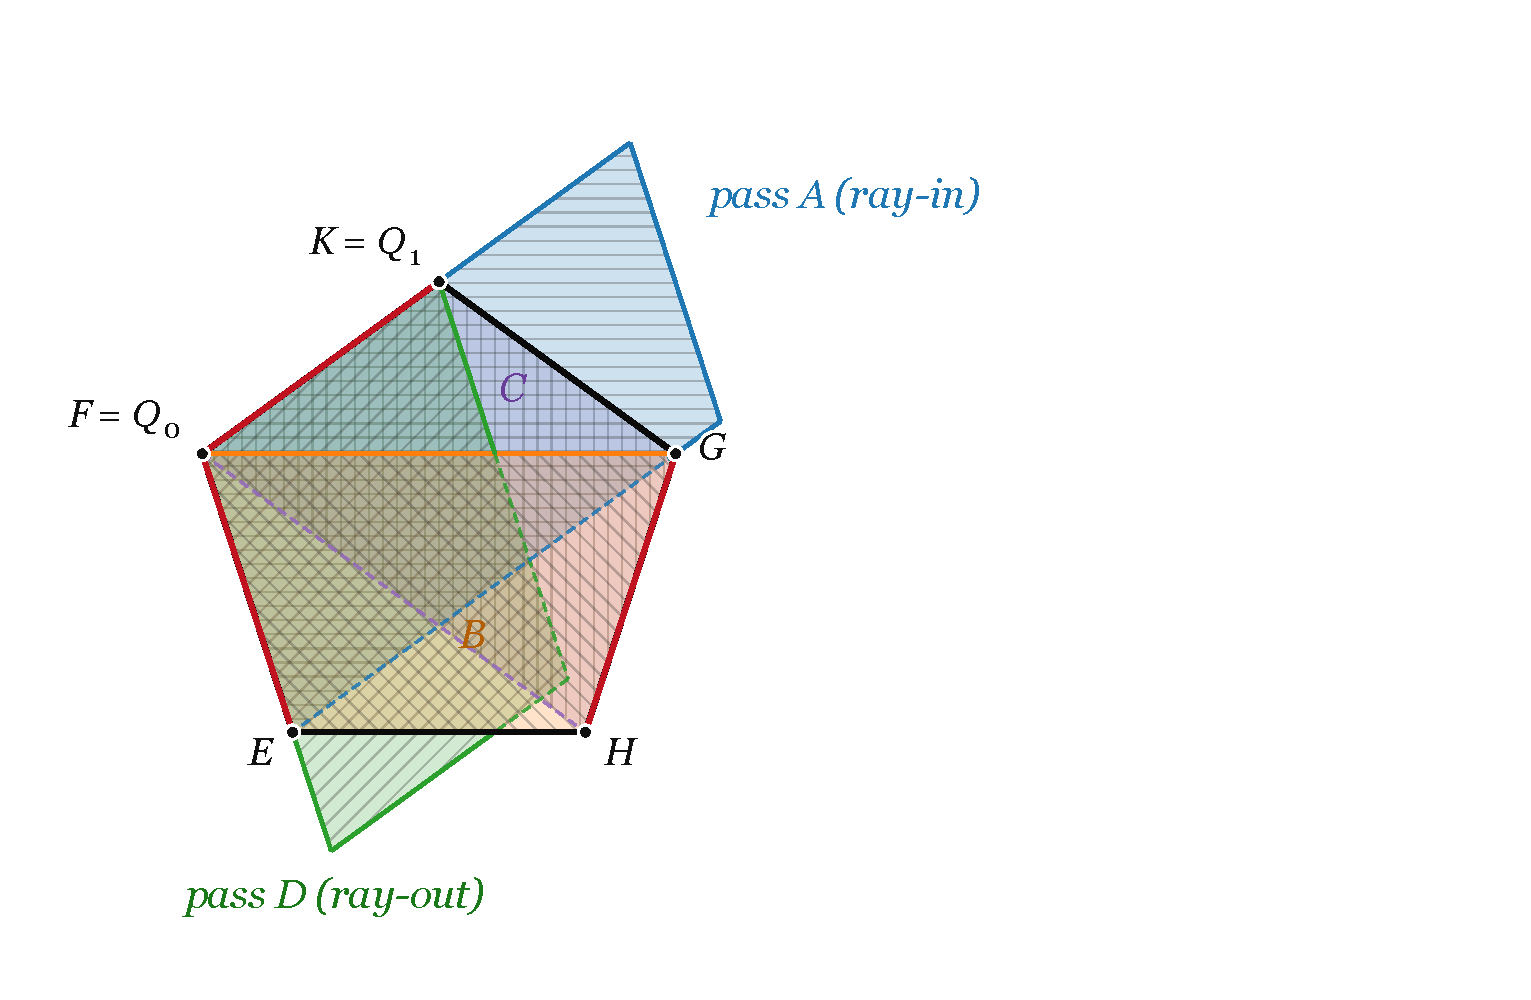
\includegraphics[width=0.92\linewidth]{figs/fig1-pentagon.pdf}
\caption{The folklore state $P^*$, drawn from the exact slice coordinates and rendered in the hidden-line convention: solid edges are visible, dashed edges pass beneath, under the layer order $B>D>A>C$. The creases are the heavy red chords, the regular pentagon $EHGKF$ is drawn in bold, and the two rays record the tying.}
\label{fig:pentagon}
\end{figure}

\subsection{Layer order, cyclic local orders, and common four-pass overlap}

\begin{definition}[Crease-neighbourhood axiom]\label{def:axiom}
If a crease $\kappa$ joins the passes $P$ and $P'$, then no neighbourhood of any point of the relative interior of $\kappa$ may be covered by a pass lying strictly between $P$ and $P'$ in the layer order.
\end{definition}

The words ``of \emph{any} point of the relative interior'' are what make the axiom bite at crease endpoints, and that is where the walls of the next subsection come from.

\begin{theorem}[Crossing relations and unique global layer order]\label{thm:layer}
In any valid flat folded state with the three-crease overhand crossing pattern, the over-under relations at the three crossings are $A>C$, $D>A$, and $B>D$ (or the global reversal). Consequently, any \emph{global} total layer order on $\{A,B,C,D\}$ compatible with these crossings is uniquely $B>D>A>C$ (up to global reversal).
\end{theorem}

\begin{proof}
By Theorem~\ref{thm:foldnumber} the three crossings sit on the non-adjacent pairs $(A,C)$, $(A,D)$ and $(B,D)$. In the material passage sequence the only freedom is the order of the two crossings inside the piece $A$ and inside the piece $D$, since $B$ and $C$ are traversed once each. Imposing alternation, that is parity of passages, together with per-crossing complementarity, namely that the two passages of one crossing have opposite parity, eliminates three of the four cases:
\begin{center}
\small
\begin{tabular}{llp{0.42\linewidth}}
\hline
order in $A$ & order in $D$ & verdict\tabularnewline
\hline
$C$ first & $A$ first & \raggedright consistent: the pairs $(1,4)$, $(2,5)$, $(3,6)$ all have opposite parity\tabularnewline
$C$ first & $B$ first & \raggedright $(A,D)$ occupies positions $(2,6)$, both even\tabularnewline
$D$ first & $A$ first & \raggedright $(A,C)$ occupies positions $(2,4)$, both even\tabularnewline
$D$ first & $B$ first & \raggedright $(A,C)$ at $(2,4)$ and $(B,D)$ at $(3,5)$\tabularnewline
\hline
\end{tabular}
\end{center}
The surviving word, with the alternating assignment, yields the three local relations $A>C$, $D>A$, and $B>D$, which are acyclic and admit a unique linear extension to a global total order on $\{A,B,C,D\}$, namely $B>D>A>C$ (or its global reversal).
\end{proof}

\begin{remark}[Cyclic local layer orders and their strong realization]\label{rem:cyclic-counterexample}
Theorem~\ref{thm:layer} does \emph{not} imply that every pointwise local layer order in the sense of Definition~\ref{def:flatstate} is induced by a global total order. Take the rational working-chart state
\[
  \theta_{\mathrm{cyc}}=\bigl(\tfrac13,\,\tfrac{301}3,\,100,\,100,\,\tfrac{302}3\bigr),
  \qquad q=\tfrac13,\quad p=-\tfrac13.
\]
Its forward directions are $(-\tfrac45,-\tfrac35),(1,0),(-\tfrac45,\tfrac35),(\tfrac7{25},-\tfrac{24}{25})$, all three turn cross products equal $\tfrac35>0$, the three centreline crossings occur at distinct transverse points in material order $\mathtt{XYZXYZ}$, and all eight walls of Section~\ref{sec:moduli} are strictly positive. Yet even the four infinite width-one support bands have no triple intersection: the minimum Euclidean distance from any pairwise band intersection to a third support band is $851/40=21.275$, and distinct pairwise overlaps along each actual pass are separated longitudinally by at least $21275/936\approx22.73$ strip widths. Retaining $A>C$, $D>A$, $B>D$ at the three crossings while assigning $A>B$ on the adjacent overlap $A\cap B$ near $\kappa_1$ gives a locally consistent pointwise layer order satisfying Definition~\ref{def:axiom}, even though combining comparisons across separated plane points yields the cycle $A>B>D>A$ (indeed all $2^3=8$ adjacent-crease choices are locally consistent, only one being globally ordered).

Moreover, this cyclic local order is strongly realizable in thin slabs: fixing passes $B,C,D$ at constant heights $2\varepsilon/3,0,\varepsilon/2$, introducing on the free incoming tail $A$ over $s\in[-25,-15]$ the smooth $C^2$ isometric height transition $z(s)=\frac\varepsilon4+\frac{3\varepsilon}4 p((s+25)/10)$ paired with horizontal arc-length parameter $S'(s)=\sqrt{1-(z'(s))^2}$ (where $p(t)=10t^3-15t^4+6t^5$, so $|z'(s)|\le\frac{9}{64}\varepsilon$ and the total horizontal foreshortening $\int_{-25}^{-15}(1-\sqrt{1-(z')^2})\,ds\le\frac{405}{2048}\varepsilon^2$ is absorbed along the free ray while all three \emph{reference flat creases} stay fixed), and joining each crease by a semicircular hairpin of radius $r$ (whose rounded material-crease midpoint projects at distance $(\pi/2-1)r$ from its reference crease, within the strong-realization tolerance) yields a strong $\varepsilon$-realization of $\theta_{\mathrm{cyc}}$ for all $0<\varepsilon\le 1/100$ with uniform projection constant $C=1$, collar constant $C_{\mathrm{ram}}=2$, sheet separation at least $\varepsilon/6$, and the same alternating trefoil knot type. The rational band separations, longitudinal overlap gaps, free-tail ramp clearance, and ramp derivative/foreshortening bounds are certified exactly in \texttt{exact\_common\_overlap}. Accordingly, the global total order $B>D>A>C$ is an explicit part of the definition of the globally ordered branch $\mathcal B$ used in Theorems~\ref{mainthm:moduli}, \ref{mainthm:realization}, and~\ref{mainthm:census}.
\end{remark}

\begin{lemma}[Common four-pass overlap forces the global order]\label{lem:common-overlap}
Suppose $(f_\theta,\lambda)$ is a flat folded state with the overhand crossing pattern and crossing relations $A>C$, $D>A$, $B>D$, whose pointwise local layer order $\lambda$ is locally constant on each pairwise pass overlap. If there exists a plane point $P$ lying strictly in the interior of all four passes $A,B,C,D$, then $\lambda$ is forced to coincide with the global total order $B>D>A>C$ on every pairwise overlap meeting $P$. This hypothesis holds:
\begin{enumerate}
\item[(i)] throughout the standard slice $0<x<1/\sqrt3$, at the point $P(x)=\bigl(\frac{h(x)}{2},\frac34\bigr)$;
\item[(ii)] at the regular pentagon $P^*$, at $\td$, on a coordinate cube of radius $10^{-3}$ around each, and along the entire certified second-family arc $[x^\dagger,x_0]$ together with its coordinate tube of radius $10^{-4}$, at the fixed point $P=\bigl(\frac12,\frac34\bigr)$.
\end{enumerate}
Consequently, the local optimality and certified-path results of Theorems~\textup{\ref{mainthm:pass}}--\textup{\ref{mainthm:kauffman}} hold under purely pointwise local layer order without assuming a global order \emph{a priori}.
\end{lemma}

\begin{proof}
Each pass image is convex, so each pairwise interior overlap $A^\circ\cap C^\circ$, $A^\circ\cap D^\circ$, $B^\circ\cap D^\circ$ is convex and hence connected. Local constancy of the relative order transports the three crossing relations $A>C$, $D>A$, $B>D$ from the three crossing points to the common interior point $P$. Because $\lambda$ is a linear order on the four material preimages over $P$, transitivity at $P$ forces $B>D>A>C$ at $P$, and local constancy on each connected pairwise overlap carries those relations to every pair overlapping at $P$.

For \textup{(i)}, evaluating the fourteen inward half-plane functionals of the four crease-bounded passes at $P(x)=(h(x)/2,3/4)$ on the standard slice \eqref{eq:slice} yields rational functions whose nontrivial numerators are $1+x^2-4x^4$, $3+6x^2-5x^4$, and $3x^2\pm2x+1$, all strictly positive on $0<x<1/\sqrt3$. For \textup{(ii)}, exact Sturm counts show that $N_5(x,1.035)$ and $N_5(x,1.053)$ have no roots on $[0.322,0.325]\supset[x^\dagger,x_0]$, confining the second-family branch to $h\in(1.035,1.053)$; outward-rounded interval evaluation of all fourteen half-plane functionals at $(1/2,3/4)$ over the $10^{-3}$ cubes around $P^*$ and $\td$ and over $192$ sub-boxes covering $[0.322,0.325]\times[1.035,1.053]$ thickened by $10^{-4}$ in all five coordinates certifies strict interior membership throughout (all interval lower bounds strictly above $0.05$, \texttt{exact\_common\_overlap}).
\end{proof}

\begin{corollary}[Prohibition lists]\label{cor:btw}
On the globally ordered branch $\mathcal B$ (with total order $B>D>A>C$), the sets of passes lying strictly between the two sides of a crease, as in Definition~\textup{\ref{def:axiom}}, are $\mathrm{Btw}(\kappa_1)=\{D\}$, $\mathrm{Btw}(\kappa_2)=\{A,D\}$ and $\mathrm{Btw}(\kappa_3)=\{A\}$.
\end{corollary}

\subsection{The walls}

Every codimension-one component of the non-penetration boundary of $\M$ is either a crease-endpoint sliver contact or a taco contact. This is not an empirical inventory but a consequence of convexity, and the following lemma is what closes it.

\begin{lemma}[Completeness of the contact catalogue]\label{lem:wallcat}
Fix a forbidden pair $(\kappa,P)$ with $P\in\mathrm{Btw}(\kappa)$, where $\kappa$ is a crease chord and $\bar P$ is the closed image of the pass, a convex polygon, possibly unbounded. Along any continuous path of states on which $\mathrm{relint}(\kappa)\cap P^\circ$ passes from empty to nonempty, the transition state satisfies, one of:
\textup{(i)} an endpoint of $\kappa$ lies on $\partial P$; or
\textup{(ii)} a vertex of $\bar P$ lies on $\kappa$.
Since every vertex of a pass image is the image of a crease endpoint, events of type \textup{(ii)} are crease-pair contacts. Consequently every codimension-one component of the non-penetration boundary is an endpoint sliver or a crease-pair contact.
\end{lemma}

\begin{proof}
At the transition state one has $\kappa\cap\bar P\ne\emptyset$, by taking a limit of intersection points from the violating side, while $\mathrm{relint}(\kappa)\cap P^\circ=\emptyset$. Pick $p\in\kappa\cap\bar P$. Suppose first $p\in\mathrm{relint}(\kappa)$; then $p\notin P^\circ$, so $p\in\partial P$. If $p$ lay in the relative interior of an edge $e$ of $\bar P$, the defining inequalities of all other edges would be strict at $p$, so near $p$ the set $\bar P$ coincides with the closed half-plane of $e$; if $\kappa$ is not parallel to $e$, it crosses the line of $e$ transversally, placing nearby relative-interior points in $P^\circ$, a contradiction. If it is parallel, the contact is collinear. The closed interval $\kappa\cap e$ then has an endpoint that is an endpoint of $\kappa$ or an endpoint of $e$ (also when $e$ is a ray or a line). These give \textup{(i)} and \textup{(ii)}, respectively. If $p$ was a vertex to begin with, \textup{(ii)} holds directly. Otherwise every point of $\kappa\cap\bar P$ is an endpoint of $\kappa$; such an endpoint cannot lie in $P^\circ$, since openness would force nearby relative-interior points of $\kappa$ into $P^\circ$, so it lies on $\partial P$, which is case \textup{(i)}.
\end{proof}

\begin{corollary}[The wall catalogue of the overhand branch]\label{cor:wallcomplete}
Within the stated working chart, the non-penetration boundary of the honest moduli $\M_{\mathrm{hon}}$ consists exactly of the six sliver walls of Table~\textup{\ref{tab:walls}} together with the windowed taco faces $\{t=1,\,0\le u\le1\}$ and $\{u=1,\,0\le t\le1\}$; the computational chamber $\Mhat$ is cut out by the same six slivers together with the unwindowed faces $\{w_9=0,\,w_{10}\le0\}$, $\{w_{10}=0,\,w_9\le0\}$ of \eqref{eq:taco}, whose extensions beyond the windows are capture faces and bound no contact.
\end{corollary}

\begin{proof}
The forbidden pairs are those of Corollary~\ref{cor:btw}, giving eight candidate endpoint events of type \textup{(i)}: both endpoints for each of $(\kappa_1,D)$, $(\kappa_2,A)$, $(\kappa_2,D)$, $(\kappa_3,A)$. Six of them are the walls of Table~\ref{tab:walls}. The remaining two, the $H$-endpoint of $\kappa_2$ against $A$ and the $G$-endpoint of $\kappa_2$ against $D$, degenerate: in the normalization \eqref{eq:coords}, with $d_2=((x^2-1),-2x)/(1+x^2)$, the band containing $A$ satisfies $0\le\operatorname{cross}(P-E,d_2)\le1$, whereas $\operatorname{cross}(H-E,d_2)=-2hx/(1+x^2)<0$. Thus $H$ is strictly outside this band on the positive chart, rather than on its carrier line. Material reversal gives the analogous strict exclusion of $G$ from the band of $D$. Adjacent crease contacts are excluded by the positive material chord distance of the intervening panel (Proposition~\ref{prop:axred}). Events of type \textup{(ii)} are crease-pair contacts; adjacent pairs are excluded by the same distance argument, leaving the pair $(\kappa_1,\kappa_3)$, whose codimension-one events are endpoint-on-segment incidences of the two crease segments. Two of the four, $F\in\kappa_3$ and $Q_0\in\kappa_1$, are exactly the taco faces $\{w_9=0,\,w_{10}\le0\}$ and $\{w_{10}=0,\,w_9\le0\}$ of \eqref{eq:taco}, by Observation~\ref{obs:corner}; the remaining two, $E\in\kappa_3$ and $Q_1\in\kappa_1$, never occur on the chart, by Lemma~\ref{lem:tacoent}(ii).
\end{proof}

With the sign convention that the feasible side is $\ge0$, the six sliver walls are those of Table~\ref{tab:walls};\footnote{The numbering is inherited from a longer preliminary list; the conditions originally labelled $w_2,w_3$ proved to be consequences of the others and are not walls. We keep the labels to stay aligned with the ancillary material.} each is the analytic statement that a particular pass fails to cover a neighbourhood of a particular crease endpoint. Because these conditions concern the endpoints of a relative interior, they must be evaluated analytically and never by sampling along the crease; see Remark~\ref{rem:methods}.

\begin{table}[t]
\centering\small
\begin{tabular}{lp{0.28\linewidth}p{0.42\linewidth}}
\hline
wall & \raggedright analytic meaning & \raggedright event forbidden by Definition~\ref{def:axiom}\tabularnewline
\hline
$w_1$ & \raggedright endpoint $G$ of $\kappa_2$ inside the lay-in band & \raggedright $A$ covers the $G$-side sliver of $\kappa_2$\tabularnewline
$w_4$ & \raggedright endpoint $H$ of $\kappa_2$ inside the lay-out band & \raggedright $D$ covers the $H$-side sliver of $\kappa_2$\tabularnewline
$w_5$ & \raggedright $\Delta\ge0$: $K$ at or beyond $I$ along $r$ on $\ell_2$ & \raggedright $A$ covers a neighbourhood of $\kappa_3$\tabularnewline
$w_6$ & \raggedright the mirror of $w_5$ & \raggedright $D$ covers a neighbourhood of $\kappa_1$\tabularnewline
$w_7$ & \raggedright $Q_0$ not beyond the far edge $e_B$ of the lay-in band & \raggedright $A$ covers the $Q_0$-side sliver of $\kappa_3$\tabularnewline
$w_8$ & \raggedright $F$ not beyond the far edge of the lay-out band & \raggedright $D$ covers the $F$-side sliver of $\kappa_1$\tabularnewline
\hline
\end{tabular}
\caption{The six endpoint-sliver walls of $\M$ in the normalization \eqref{eq:coords}. Each is a corner-on-edge contact, a crease endpoint of one pass meeting the boundary of another.}
\label{tab:walls}
\end{table}

The remaining boundary has a different logical shape. Let $E+t(F-E)=Q_1+u(Q_0-Q_1)$ be the intersection of the \emph{lines} carrying $\kappa_1$ and $\kappa_3$, and set $w_9=t-1$ and $w_{10}=u-1$. The forbidden event is that the two crease \emph{segments} cross in their relative interiors---the taco--taco prohibition of flat origami \cite{justin1997}---that is
\[0<t<1\quad\text{and}\quad 0<u<1\quad\text{simultaneously}.\]
The lower bounds are not additional walls: they are governed by an exact linear entanglement of the pair.

\begin{lemma}[Entanglement of the taco pair]\label{lem:tacoent}
Write $q=g-h$, $W_0=(1+q^2)w_0=(q^2-1,2q)$, $\alpha=2aq/(q^2+1)$ and $\beta=2bq/(q^2+1)$, so that the endpoints of $\kappa_3$ sit at heights $y(Q_1)=1+\alpha$ and $y(Q_0)=\beta$. On the chart, where $h,a,q>0$:
\begin{enumerate}
\item the identity $t-1=\alpha(1-u)+u\,(\beta-1)$ holds, the height along the line of $\kappa_3$ taking the value $t$ at the intersection point;
\item the endpoint events $E\in\kappa_3$ and $Q_1\in\kappa_1$ never occur: $\kappa_3$ lies in the closed band of $C$, whose $H$-side edge line has $E$ strictly on its far side, by $\operatorname{cross}(E-H,W_0)=-2hq<0$ against the band-side value $\operatorname{cross}(G-H,W_0)=q^2+1>0$; and $y(Q_1)=1+\alpha>1\ge\max_{\kappa_1}y$;
\item on $\{\beta\ge1\}$ the forbidden event is impossible: $0<u<1$ forces $t-1=\alpha(1-u)+u(\beta-1)>0$;
\item $\beta\equiv1$ on the standard slice, where $Q_0=F$ identically; on the certified segment of the second family from $P^*$ to $\td$, one has $\beta>1$ away from $P^*$ and $1+\alpha-\beta>0$ throughout, by root-free resultants with $N_5$ and exact sign anchors, the pentagon endpoint factor of $\beta-1$ deflating exactly; at $P^*$, $\beta=1$ and $\alpha=(\sqrt5-1)/2=\varphi^{-1}$; at $\td$, $t-1=u-1\approx0.0506$ and $\beta-1\approx0.0796$, both certified positive in $\Q[x]/(p_x)$; and along this segment $t=u=(1+x^2-2hx)/(4x^2)$ in closed form. Certificate \texttt{exact\_taco} \cite{anc}.
\end{enumerate}
\end{lemma}

On $\{t>0\}\cap\{u>0\}$ the complement of the forbidden event is therefore exactly the union
\begin{equation}\label{eq:taco}
  \{w_9\ge0\}\cup\{w_{10}\ge0\},
\end{equation}
while on $\{t\le0\}\cup\{u\le0\}$ the prohibition is vacuous and \eqref{eq:taco} is a strengthening. Three spaces organize the discussion. $\Mhon$ is the moduli with the honest prohibition. $\Mplus:=\Mhon\cap\{t>0,\,u>0\}$ is the \emph{positive-taco moduli}, on which the honest prohibition coincides exactly with the disjunction \eqref{eq:taco}. $\Mhat$ is the \emph{computational chamber}: the semialgebraic set cut out by the sliver walls and the unwindowed disjunction \eqref{eq:taco}, with no positivity requirement on $(t,u)$. Then
\[\Mplus\;=\;\Mhat\cap\{t>0,\,u>0\}\;\subseteq\;\Mhat\;\subseteq\;\Mhon,\]
the second inclusion because \eqref{eq:taco} implies the honest prohibition outright. Every state at which this paper runs a first- or second-order analysis---the standard slice, both one-parameter families, $P^*$, and $\td$---lies in $\Mplus$ with margins certified by Lemma~\ref{lem:tacoent}(iv), and near those states the three spaces agree: the far pieces $\{t\le0\}\cup\{u\le0\}$ are empty in a neighbourhood, so \eqref{eq:taco} \emph{is} the segment-crossing prohibition there. Throughout, the working symbol $\M$ denotes the chamber $\Mhat$: every existence, reachability, and path statement proved in $\M$ holds verbatim in $\Mhon$, the local theorems may be read in $\Mplus$ unchanged, and the census of Section~\ref{sec:census} runs over $\Mhat$, whose faces beyond the windows are \emph{capture faces}---constraint extensions, not non-penetration walls. The stratified census of Section~\ref{sec:census} is likewise unaffected: its recorded exclusion verdicts rest on sliver-wall signs and Krawczyk isolation alone, never on the taco pair. The honest catalogue is also settled by the same lemma: a path of honest states entering the forbidden box must cross its boundary, the entry faces $\{t=0,\,0\le u\le1\}$ and $\{u=0,\,0\le t\le1\}$ are empty by Lemma~\ref{lem:tacoent}(ii), so the honest non-penetration boundary consists of the six slivers together with the \emph{windowed} taco faces $\{t=1,\,0\le u\le1\}$ and $\{u=1,\,0\le t\le1\}$; the chamber's faces extend these beyond the windows, and the extensions $\{t=1,\,u<0\}$, $\{u=1,\,t<0\}$ separate two honestly-valid regions and bound no contact. The union \eqref{eq:taco} is not convex. We call $w_9,w_{10}$ the \emph{taco pair}: the forbidden event is two creases folding shut on one another. First-order blocking tests must therefore be run separately on the two branches $\{w_1,\dots,w_8,w_9\}$ and $\{w_1,\dots,w_8,w_{10}\}$; on each branch the constraint system is an ordinary linear one, and Carath\'eodory's theorem makes the enumeration of basic solutions a complete decision procedure \cite{barvinok2002,nocedal2006}.

\begin{observation}[The taco walls are corner contacts]\label{obs:corner}
One has $w_9=w_{10}=0$ if and only if $Q_0=F$. Indeed $t=1$ places the intersection of the two crease lines at $F$ and $u=1$ places it at $Q_0$. The locus $\mathcal F=\{Q_0=F\}$ is cut out by two equations and is a three-dimensional submanifold of $\M$; its intersection with $\{w_1=w_4=0\}$ is exactly the standard slice, on which all six of $w_1,w_4,w_7,w_8,w_9,w_{10}$ vanish identically. The taco pair is thus not a self-intersection of a pass but a corner contact of the crease pair $\kappa_1,\kappa_3$.
\end{observation}

\begin{proposition}[Stratification]\label{prop:strat}
Inside the fixed nondegenerate branch chart, the relative closure of $\M$ is semialgebraic and is stratified by the active constraint set; the full closure in $\R^5$ acquires, in addition, code and general-position degeneration faces---branch-exit events, open conditions in the branch datum, not part of the wall stratification. The standard slice is exactly $\{w_1=w_4=w_7=w_8=0\}$, the four contact equations of the classical slice construction being equivalent to the activation of these four walls, and the regular pentagon is the unique point at which all eight walls, sliver and taco alike, are active. Two further contact functions, incidence of $F$ with an edge and passage of $\kappa_3$ through $F$, are not walls but stratum labels, since both signs occur among valid states.
\end{proposition}

\begin{proof}
Semialgebraicity is immediate, every wall function being rational with integer-coefficient numerator and denominator; denominators are nonzero with fixed signs on each chart component. The identification of the standard slice with $\{w_1=w_4=w_7=w_8=0\}$, the simultaneous activity of all eight sliver and taco walls at the regular pentagon and at no other point, and the occurrence of both signs of the two discarded contact functions are direct computations, verified in exact arithmetic in the ancillary suite \cite{anc}.
\end{proof}

\begin{proposition}[Axiom reduction]\label{prop:axred}
On the globally ordered overhand branch $\mathcal B$, the crossing datum determines the unique global layer order $B>D>A>C$ \textup{(Theorem~\ref{thm:layer})}, and that global order together with Definition~\textup{\ref{def:axiom}} implies the transversality clause of crease-pair non-crossing. Hence within $\mathcal B$ the only logically independent axioms are the crease-neighbourhood axiom and the branch datum (including the global layer order).
\end{proposition}

\begin{proof}
Adjacent crease pairs cannot meet at all, since the distances $d(\kappa_1,\kappa_2)$ and $d(\kappa_2,\kappa_3)$ equal the corresponding material chord distances, which are positive by rigidity of the intervening panel. If $\kappa_1$ and $\kappa_3$ crossed transversally in their relative interiors, then a relative interior point of $\kappa_1$ next to the crossing would lie in the interior of the image of $D$, and $D\in\mathrm{Btw}(\kappa_1)$ by Corollary~\ref{cor:btw}, violating Definition~\ref{def:axiom}. Collinear overlap of two creases is not covered by this argument, since in that degenerate case $D$ covers only a half-neighbourhood; it is excluded here by the explicit nonparallel-crease condition of the working chart, not by centreline general position. No conclusion for parallel crease pairs follows from this argument.
\end{proof}

Proposition~\ref{prop:dim}, Theorem~\ref{thm:layer}, Lemma~\ref{lem:wallcat}, Corollary~\ref{cor:wallcomplete}, Observation~\ref{obs:corner} and Propositions~\ref{prop:strat} and~\ref{prop:axred} together constitute Theorem~\ref{mainthm:moduli}.

\begin{remark}[Status of the classification]\label{rem:wallsnum}
Lemma~\ref{lem:wallcat} and Corollary~\ref{cor:wallcomplete} give the complete wall list. Exact witnesses of both signs show that the two stratum labels of Proposition~\ref{prop:strat} bound no face. The ancillary material \cite{anc} includes these witnesses, the endpoint criteria and supplementary numerical boundary sweeps.
\end{remark}

\section{Tightening and the pentagonal junction}\label{sec:tightening}

\subsection{The functional of pulling}

\begin{definition}[Core length]\label{def:core}
Let $m_1<\cdots<m_n$ be the material points at which the centreline meets the creases and let $M_i$ be their images. The \emph{core length} is
\[
  \core=m_n-m_1=\sum_{i=1}^{n-1}|M_iM_{i+1}| ,
\]
the material trapped between the first and the last crease; the second equality holds because panels are rigid.
\end{definition}

\begin{proposition}[Why this is the functional of pulling]\label{prop:pulling}
On a finite strip of length $L$ the two tails have total material length $L-\core$. Hence extracting as much tail as possible and minimizing $\core$ are the same problem, and only the latter survives the passage to long strips.
\end{proposition}

This is where the model parts company with Kauffman's truncation length $\trunc$ \cite{kauffman2004}, which measures the material needed to \emph{build} the flat knot rather than the material that pulling extracts. Both are natural, both are defined on the same moduli space, and the sequel shows that they select different strict local optima.

\begin{definition}[Pulling path and tight state]\label{def:pull}
A \emph{pulling path} is a continuous path $p\colon[0,1]\to\overline{\M}$ which satisfies non-penetration at all times while preserving the branch, so that crumpling and layer rearrangement are excluded by definition, and along which $\core\circ p$ is non-increasing. A state reachable from a slack state, one at which all contact inequalities are strict, is \emph{tight} if no pulling path issuing from it strictly decreases $\core$.
\end{definition}

This is the path version of a constrained local minimum. It combines the contact-force characterization familiar from ropelength criticality \cite{cks2002,svdm2004} with the monotone-path formulation used for expansive motions \cite{cdr2003}; the balance between the gradient of the objective and the active wall gradients that appears below is the folded analogue of the vertex tension balance of the immersed theory \cite{immersed2020,ayala2025}.

\subsection{The slice theorem}

\begin{lemma}[Closed form on the slice]\label{lem:sliceform}
On the standard slice the two core segments have equal length and
\[
\begin{gathered}
  |M_1M_2|=|M_2M_3|=\frac{1-x^2}{2x},\qquad
  \core(x)=\frac{1-x^2}{x}=\frac1x-x,\\
  \core'(x)=-\frac1{x^2}-1<0 .
\end{gathered}
\]
Pulling along the slice is therefore exactly the increase of $x$.
\end{lemma}

\begin{proof}
The end exchange of the slice swaps the two core segments, so they have equal length. Substituting the values of $g$ and $h$ from \eqref{eq:slice} into $(g+h+x)/2$, the common length of the two segments, gives $(1-x^2)/(2x)$; summing and differentiating gives the remaining two identities. The computation is verified in exact arithmetic in the ancillary suite \cite{anc}.
\end{proof}

\begin{theorem}[Slice tightening]\label{thm:slice}
A pulling path confined to the standard slice $\{x\in(0,\tfrac1{\sqrt3})\}$ has feasible region $\{\Delta(x)\ge0\}=(0,x_0]$ and a unique tight state, at $x=x_0=\sqrt{1-2/\sqrt5}$: the regular pentagon.
\end{theorem}

\begin{proof}
The slice is one-dimensional with parameter $x$ by Proposition~\ref{prop:strat}. The gap $\Delta=k-\mu$ of \eqref{eq:slice} is strictly decreasing with a unique zero $x_0$ in $(0,\tfrac1{\sqrt3})$; strict decrease follows from the sum-of-squares identity
\[
  5x^6-5x^4+7x^2+1=5x^2\Bigl(x^2-\tfrac12\Bigr)^2+\tfrac{23}4x^2+1>0
\]
for the numerator of $\Delta'$. Since $\core$ is strictly decreasing by Lemma~\ref{lem:sliceform}, a pulling path can only increase $x$, and at $x_0$ the wall $w_5$, that is $\Delta=0$, equivalently $K=I$, equivalently $\kappa_3$ flush with the far edge $e_B$, becomes active. For $x<x_0$ a further increase is possible, so no earlier point is tight.
\end{proof}

At $x_0$ all five sides of the central polygon $E,H,G,K,F$ have equal length, with $|EH|^2=2-\tfrac{2\sqrt5}5$, all five interior angles have cosine $-\tfrac{\sqrt5-1}4=\cos108^\circ$, and the two tails make an angle of $72^\circ$. These are exact identities in $\Q(\sqrt5)$, checked by the symbolic geometry scripts. Lean~4 checks supporting algebraic identities, including $|EH|^2=|EF|^2$ under the contact equation and a positivity identity proving the monotonicity of $\Delta$; it does not formalize the polygon or its five angles \cite{mathlib2020,anc}. The five sides are precisely the three creases and two band edges: the pentagon is not an approximation but the exact contact-limited endpoint of the slice, which is the folklore statement, proved.

\subsection{Tightening cannot stop in the interior}

\begin{proposition}[Affine core length and no interior critical point]\label{prop:nointerior}
On the forward chart, where $g+h+x>0$ and $a+b>0$,
\[
  \core(\theta)=\frac{x+g+h+a+b}{2},\qquad
  \nabla\core=\tfrac12\mathbf1,\qquad \nabla^2\core=0.
\]
In particular there is no interior critical point.
\end{proposition}

\begin{proof}
An isometry takes the midpoint of a complete material crease chord to its centreline fold point. Thus
$M_1=(-x/2,1/2)$, $M_2=((g+h)/2,1/2)$, and
\[
M_3=\frac{Q_1+Q_0}{2}=M_2+\frac{a+b}{2}\,w_0.
\]
Since $|w_0|=1$, the two forward centreline segments have lengths $(g+h+x)/2$ and $(a+b)/2$. Adding and differentiating proves the claim. Without the forward assumptions the respective absolute values are required. The identity and derivative are also checked by \texttt{exact\_core\_descent}.
\end{proof}

\begin{proposition}[The gradient at the pentagon]\label{prop:gradpent}
At $P^*$, as everywhere in the forward chart, $\nabla\core=\tfrac12\mathbf1$. The equality of its five entries is a consequence of complete-chord midpoint geometry, not a special symmetry of the pentagon.
\end{proposition}
\begin{proof}
Apply Proposition~\ref{prop:nointerior}.
\end{proof}

\subsection{The pentagon is a contact-mode junction: descent passes through}

The term is descriptive; no minimax theory is invoked.

\begin{theorem}[The pentagonal contact-mode junction: descent passes through $P^*$]\label{thm:pass}
At $P^*$ all eight walls are active. For each of the two taco branches of \eqref{eq:taco} the gradient $\nabla\core$ does \emph{not} lie in the non-negative cone spanned by the active wall gradients: every basic solution has a negative multiplier, and by Carath\'eodory's theorem the test is complete. Consequently a first-order feasible descent direction exists; explicitly,
\[
  \delta^*\approx(-0.0844,\ +0.4420,\ -0.5786,\ -0.5786,\ +0.3576)
\]
keeps $w_1=w_4=w_5=w_6=0$ to first order, moves $w_7,w_8,w_9,w_{10}$ into the feasible side, and satisfies $\nabla\core\cdot\delta^*<0$. There is also a strictly inward rational descent direction
\begin{gather*}
d=10^{-6}(-163127,1000000,-883304,-887250,833681),\\
\nabla\core\cdot d=-\frac1{20}.
\end{gather*}
Every one of the eight wall derivatives is strictly positive along $d$; the first four lie between $0.0857$ and $0.0858$, and the last four between $3.199$ and $3.204$. Hence $P^*+td$ is feasible with decreasing core length for all sufficiently small $t>0$. The regular pentagon is therefore not a local minimum of $\core$.
\end{theorem}

\begin{proof}
All wall functions and $\core$ are rational in $\theta$, since reflections preserve norms and no normalization is required, so every gradient at $P^*$ is an exact element of $\Q(\sqrt5,x_0)$. The Farkas alternative is decided exactly on each branch by \texttt{exact\_farkas2}, and $\delta^*$ is a rounding of the exact solution of the four-equality system. Independently, \texttt{exact\_core\_descent} encloses each derivative along the displayed rational $d$ strictly above zero. Taylor expansion makes all eight active walls positive for small $t>0$, while the open branch conditions persist by continuity. The affine core formula makes its decrease exactly $t/20$. This supplies a nonlinear feasible path, rather than relying on tangency alone.
\end{proof}

\begin{figure}[t]
\centering
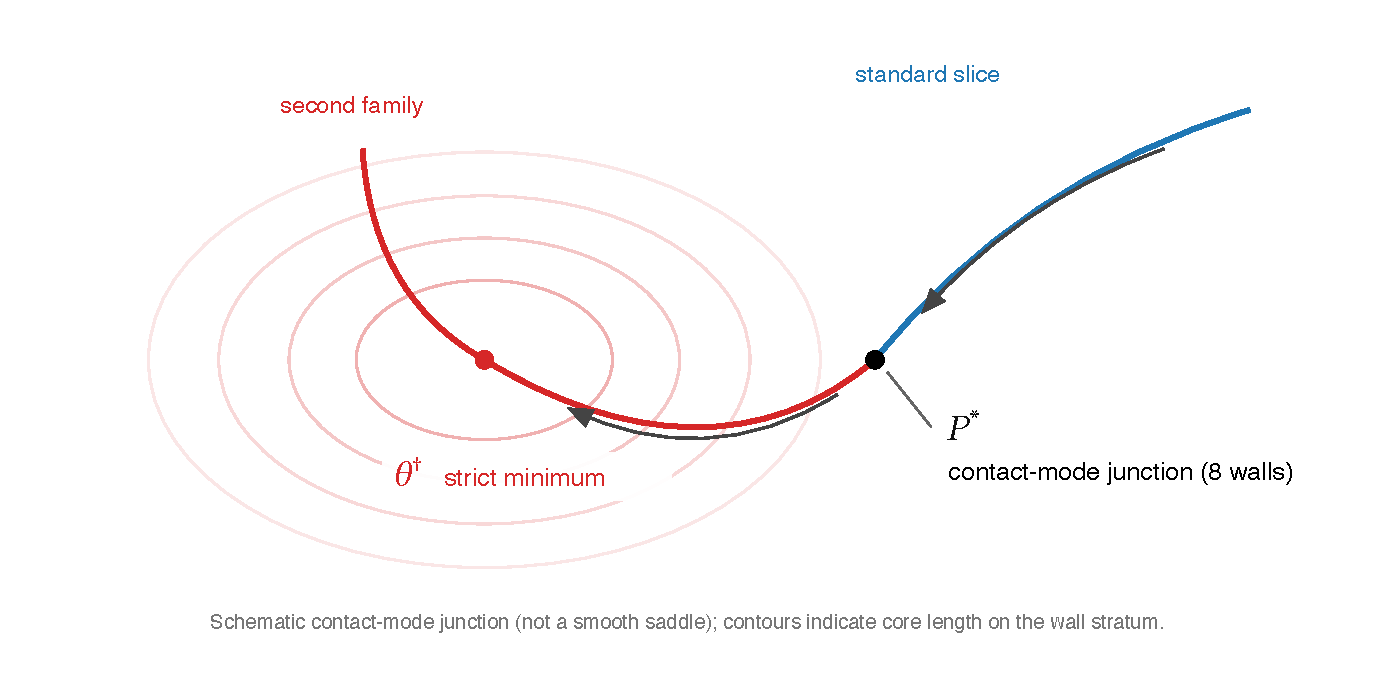
\includegraphics[width=0.92\linewidth]{figs/fig3-mountain-pass.pdf}
\caption{The regular pentagon as a contact-mode junction---informally, a mountain pass---shown schematically. The standard slice and the second symmetric family cross at $P^*$; descent of the core length passes through the crossing and continues along the second family to $\td$, feasibly and strictly monotonically by the certificates of Remark~\ref{rem:edge}.}
\label{fig:pass}
\end{figure}

\begin{proposition}[The two families and the pass]\label{prop:families}
The edge $\{w_1=w_4=w_5=w_6=0\}$ is a second mirror-symmetric one-parameter family of feasible states, the mirror symmetry surviving along it in the form $h=a$, $w_7=w_8$ and $w_9=w_{10}$, and it is distinct from the standard slice $\{w_1=w_4=w_7=w_8=0\}$. It is feasible only for $x<x_0$, since $w_7,\dots,w_{10}$ all become negative for $x>x_0$. Hence the pentagon is a common endpoint of these two distinct mirror-symmetric one-parameter families, the ones arising from the two specified symmetric active-set loci.
\end{proposition}

\begin{proof}
That the four equations cut out a one-parameter family, that the mirror symmetry survives along it in the stated form, and that the family is distinct from the standard slice are direct computations, verified in exact arithmetic in the ancillary suite \cite{anc}; the one-sided feasibility is now exact, by the certificates of Remark~\ref{rem:edge}.
\end{proof}

Geometrically, along the second family the knot releases the corner lock at $F$ and at its mirror image, so that $w_7,w_9>0$ and $w_8,w_{10}>0$, while it retains the two corner slivers $w_1,w_4$ and the two flush contacts $w_5,w_6$, and it tightens further. Theorem~\ref{thm:slice}, Theorem~\ref{thm:pass}, Proposition~\ref{prop:families} and Remark~\ref{rem:edge} together constitute Theorem~\ref{mainthm:pass}, and they turn the tightening story into a chain: the standard slice carries the classical relative tightening path inside its contact stratum, terminating at the regular pentagon, while genuine slack states reach $P^*$ along the reverse of the opening segment of Corollary~\ref{cor:slackstart}; the pentagon is passed through rather than stopped at; and descent continues along the second family to the state $\td$ analysed in the next section. Figures~\ref{fig:pass} and \ref{fig:families} display the two families and their crossing.

\begin{figure}[t]
\centering
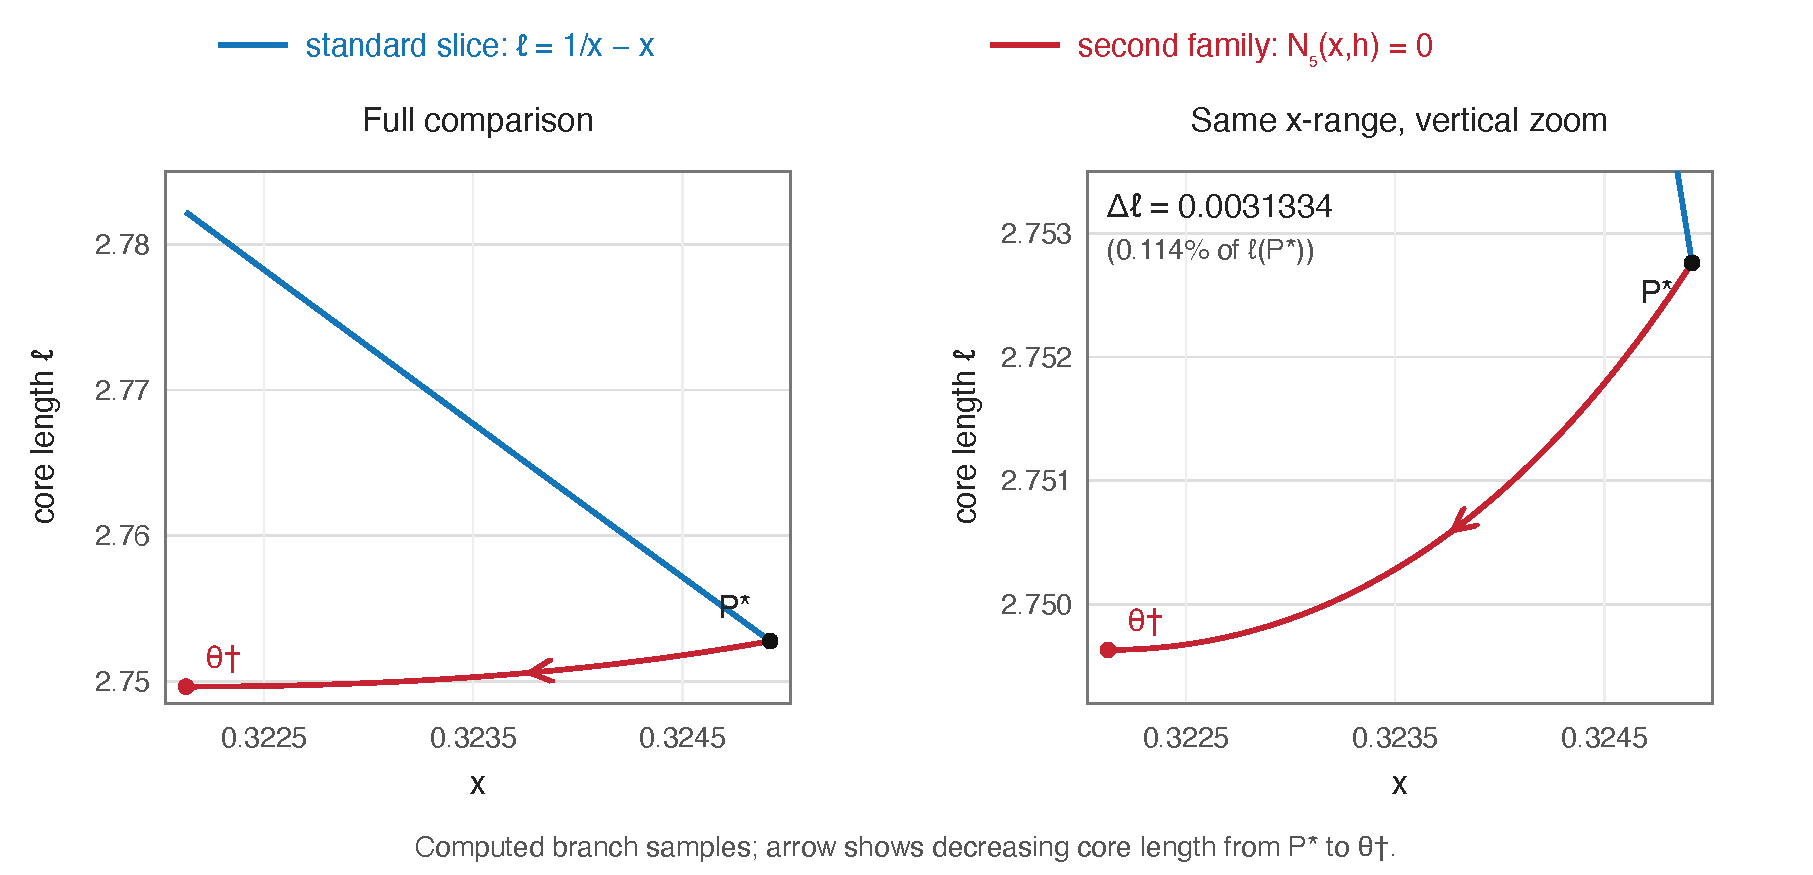
\includegraphics[width=0.92\linewidth]{figs/fig4-two-families.pdf}
\caption{The two one-parameter families in the $(x,\core)$ plane. The standard slice $\core=1/x-x$ meets the second family at $P^*$, and the second family attains its strict minimum at $\td$, below the pentagon value. Right: the same interval with an expanded vertical scale.}
\label{fig:families}
\end{figure}

\begin{remark}[Feasible monotone descent, exactly]\label{rem:edge}
Restrict the four remaining constraints to the second family. With $g$ and $b$ eliminated and $a$ replaced by $h$, each of $w_7=w_8$ and $w_9=w_{10}$ (equal in pairs, because the family lies in the mirror-fixed locus and the mirror exchanges the pairs) has a polynomial numerator in $(x,h)$ over positive denominators, and $d\core/dx$ has numerator $-K$, with $K$ the critical polynomial \eqref{eq:critpoly}, over $2x^2\,\partial_hN_5$. Exact endpoint identities hold: $K(x^\dagger,h^\dagger)\equiv0$ in $\Q[x]/(p_x)$, and at the pentagon, where $h_0^2=1+x_0^2$, the numerators of $w_7$ and $w_9$ vanish in $\Q[x]/(5x^4-10x^2+1)$. The resultants with $N_5$ of all five relevant polynomials---the two wall numerators, the taco denominator, $K$, and $\partial_hN_5$---have no real roots in $[0.322,0.325]\supset[x^\dagger,x_0]$ after removing the endpoint factors, by exact Sturm counts; the height strip of Lemma~\ref{lem:common-overlap} contains exactly one root at $x=1293/4000$, and interval Newton maps a radius-$10^{-20}$ box there strictly into its interior. The wall numerators and the taco denominator are positive at this anchor. Both $-K$ and $\partial_h N_5$ are negative, giving a positive derivative. Hence on the open interval the branch is smooth, $w_7=w_8>0$ and $w_9=w_{10}>0$, and $d\core/dx>0$ with equality only at $x^\dagger$. Descent from the pentagon along the second family therefore reaches $\td$ through valid states with strictly decreasing $\core$; the path is moreover branch-preserving, twenty-two further root-free resultants fixing the crossing pattern, passage word, and general-position margins along the whole family (Remark~\ref{rem:branchaudit}). Hence $\td$ is reachable and tight in the sense of Definition~\ref{def:pull}. The certificates are \texttt{exact\_reach} and \texttt{exact\_branch} in the ancillary suite \cite{anc}.
\end{remark}

\begin{remark}[Methods: why the certificates must be exact]\label{rem:methods}
At a sampled asymmetric state with $\core=2.6233$, the lay-in band covers a sliver of $\kappa_2$ near crease parameter $0.98$. An interior sampling grid misses the penetration, while the endpoint wall functions give $w_1=-0.061$ and $w_4=-0.062$. A second example concerns the opposite inference. A search over $400\,000$ random directions at $P^*$ found no feasible decrease. Yet the direction $d$ of Theorem~\ref{thm:pass} decreases $\core$ strictly and has positive margins on all eight walls. Its strict margins give an open cone of feasible descent directions. The tangent $\delta^*$ preserves four equalities.
\end{remark}
